\section[The Heat Pack and New Thermal Phenomena]{Making Sense of the Heat Pack: Exploring New Physical Phenomena}
\label{act1.1.5}

\begin{overview}

\noindent
{\bfseries Overview:} We return to our efforts of making sense of the heat pack by using both the \ThreePhaseModel{} and the \EnergyInteractionModel{}. In the process, we'll explore some new, related thermal phenomena -- \emph{Super-Heating} and \emph{Super-Cooling} -- and we'll see that we have to modify the standard \ThreePhaseModel{} to describe and understand the heat pack.
	
\end{overview}


\note{Timing: \unit[\about50]{min}}{
	
	\subsubsection*{Purpose}
		\begin{itemize}
			\item To provide more practice making sense of a ``strange phenomena,'' the heat pack, by applying the standard \ThreePhaseModel{} to some parts the heating and cooling cycles of a heat pack
			\item Seeing how to extend/modify the \ThreePhaseModel{} to include super-cooling
			\item Seeing how this extension of the \ThreePhaseModel{} is an example of how models start out as simple as possible and are then made more sophisticated as new data-patterns are incorporated
		\end{itemize}
	
	\subsubsection*{Learning Outcome}
		\begin{itemize}
			\item Be able to use the \ThreePhaseModel{} and the \EnergyInteractionModel{} to explain the behavior of a sodium acetate heat pack during each heating and cooling process of its entire cycle.
		\end{itemize}
}

\note{}{
	The \textbf{THEME} of this activity is to use the {\em representations of the two models}, i.e., the \EnergyDiagram{} and the \TempGraph{}, in an analytic way, rather than having ``to know the answer'' or asking the instructor The models are more than just the collection of relationships (equations); a model like these contains explicitly in the representations the procedural knowledge needed to figure out what to do next when ``you don't know what to do.'' 
}


\subsection{Taking the Heat Pack through its Entire Cycle}

\begin{fnt}
	\label{fnt1.1.3-2}

When using the \EnergyInteractionModel{} to make sense of the behavior of a heat pack (or really, any thermal cycle), it helps to divide the overall process (cycle) into multiple sub-processes.  Use the following sub-processes:

\begin{center}
\begin{tabular}{llll}
	\hline\hline
	&	Initial conditions	&	Action	&	Final Conditions\\
	\hline
	(a)	&	liquid at \unit[100]{\textdegree C}	&	taken out of boiler	&	liquid at \unit[23]{\textdegree C}\\
	(b)	&	liquid at \unit[23]{\textdegree C}	&	triggered	&	solid/liquid at \unit[54]{\textdegree C}\\&& (and insulated)	& shortly after triggering\\&&& (in mixed state)\\
	(c)	&	solid/liquid at \unit[54]{\textdegree C}	&	sitting on table	&	 solid at \unit[23]{\textdegree C}\\
	(d)	&	solid at \unit[23]{\textdegree C}	&	placed in boiler	&	solid/liquid at \unit[54]{\textdegree C}\\
	(e)	&	solid/liquid at \unit[54]{\textdegree C}	&	left in boiler	&	liquid at \unit[100]{\textdegree C}\\
	\hline\hline
\end{tabular}
\end{center}

\noindent Make four \EnergyDiagrams{}, one for each sub-process (a), (c), (d), and (e), but NOT (b). Also, make a \TempGraph{} for each process. Make sure you can describe each process {\em in your own words} using both of the representations. 
\end{fnt}

%\subsection*{\em All members of your group must now go to the board and work on the following together.}

\note{}{
	This really does work best if the whole group is up at the board. This is one of the most effective ways to encourage discussion between the members of the small groups. Keep encouraging students to just stand at the board at all times instead of going back and forth between sitting in chairs and standing at the board...
}

\note{General directions}{
	\begin{itemize}
		\item Assign one part of this FNT to each group to put on the board \textbf{BUT NOT part (b) yet!} These parts: (a), (c), (d), and (e) are pretty straightforward. Make sure the students are clearly specifying the interval, getting the indicators correct, and writing the algebraic equation for energy conservation as
		\item $\Delta E_\text{system} = Q$  and the open \EnergyDiagram{} shows Heat (the word, not the symbol ``$Q$'') with an arrow pointing in or out as appropriate.  The symbol ``$Q$'' is a signed variable, so it can be confusing for the better students, who recognize this to have arrow pointing in either direction
	\end{itemize}
}

	\noindent{\bfseries Very important for the following}: Make sure everyone in your group is ready to {\em explain} to the whole class \textbf{\em how} they know the answers to the following questions (detailed instructions below):

\begin{enumerate}

	\item Does each energy system increase or decrease?
	\item Is this an open or closed system with respect to energy, and if open, does energy come in or leave?
	\item How are your responses consistent with your \TempGraph{}?
	\item And finally, how do both diagrams tell you about the sign of each term in the equation expressing energy conservation?
	
\end{enumerate}

	\noindent To make this task a bit more manageable, your instructor will assign one of the four heat pack processes listed in \ref{fnt1.1.3-2} to your group:  (a), (c), (d), or (e) -- note that we're not concerned with Part (b) yet. For your assigned process, put on the board both 
	\begin{enumerate}[(i)]
		\item a \TempGraph{},
		
	{\bfseries and}
		
		\item an \EnergyDiagram{}.
	\end{enumerate}
	
	\noindent{\bfseries Make sure that} the two representations of the process are in agreement and that everyone in your group can explain why they are drawn the way they are. Refer to ``Steps Involved in Using the \EnergyDiagram'' on the model summary page. 

\WCD

\note{}{
	\begin{itemize}
		\item To keep this short, they don't need to explain how they constructed the entire diagram, but give the WC the opportunity to ask them about any questions they have.
		
		\item Definitely have each SG explain how they know whether each energy system in their diagram increases or decreases, and what that tells them about the sign of each term in their algebraic expression of energy conservation.
		
		[\textbf{Why is this important?} Many students fail to realize that the \EnergyDiagram{} can give knowledge ({\em with absolute certainty}) of the algebraic sign of each $\Delta E$ term.  This needs to be stressed repeatedly to the students because the great majority of them have (largely unconsciously) adopted the strategy: ``find and plug into an equation!'']
		
		\item Also stress that the \TempGraphs{} MUST agree with the \EnergyDiagram{} if there is any energy in or out.
	\end{itemize}
}

\subsection[The Clicking Mystery]{The Clicking Mystery: Super-heating and super-cooling}

\noindent
As we'll find out here, we have to modify the standard \ThreePhaseModel{} to illustrate what happens in the heat pack. Let's start with some preparations in this FNT.

\begin{fnt}
	\label{fnt1.1.3-3}

We want to analyze triggering step (b) in \hyperref[fnt1.1.3-2]{\thefnt} more closely using the \TempGraph{} of the \ThreePhaseModel{}. This will help us get a deeper understanding of this part of the process and will enable us to extend the \ThreePhaseModel{} to make it more realistically explain actual phenomena. (It turns out that super cooling and super-heating are rather common. Usually, however, they occur over a very small temperature range and so go unnoticed.)

\begin{enumerate}
	\item Sketch a \TempGraph{} for sodium acetate between room temperature at approximately \unit[150]{\textdegree C}, assuming the sodium acetate does not undergo any super-cooling, i.e., assuming that the heat pack is solid at room temperature, and changes phase at its normal phase change temperature, which you determined in \hyperref[act1.1.2]{Activity~\ref*{act1.1.2}}.
	
	\item On the same diagram, sketch the path representing the process of the liquid heat pack cooling down from \unit[150]{\textdegree C} to room temperature with no phase change (now assuming there is supercooling). Check that the path you sketched makes sense by verifying that the changes in temperature and energy shown on the diagram as you move along the path you sketched match what you know about the actual changes in temperature and energy of the heat pack as it cools to room temperature without changing phase from liquid to solid.
\end{enumerate}
\end{fnt}

\note{General directions}{
	Try to get most of their mistakes cleared up {\em before} the Whole Class Discussion. As they put up diagrams that have mistakes, instead of just telling them what is wrong, have them ``interpret'' what they have diagrammed by having them {\em start at the initial state} on the diagram and tell you what their diagram is describing {\em as the process proceeds}. Then ask them if that description matches the process in the FNT. [The lead instructor should explain this strategy]
	
	Make sure every group ends up with the correct combined graphs on their board, since they will need this for the next part.  The cooling curve is one diagonal straight line.  The heating curve is identical from 54 to \unit[100]{\textdegree C} and on top of the first curve, but at \unit[54]{\textdegree C} it has a horizontal section, which displaces the lower diagonal part to the left.
}

\begin{benumerate}

	\bitem{Extending the \TempGraph{}}
	
	Now you are going to take the two paths from \ref{fnt1.1.3-3}, and draw them ``on top of each other.'' The trick is to figure out where they exactly overlap and where the two paths deviate from each other.
	
	Erase your board and draw, fairly large, the \TempGraph{} that you drew for process A in \ref{fnt1.1.3-2}: Cooling from \unit[100]{\textdegree C} to \unit[23]{\textdegree C} with no phase change.
	
	Now, we are going to draw the combined heating process (d) plus (e) in the same diagram. \textbf{BUT WAIT!} The heating curve you draw will need to be ``on top of one another'' \textbf{where they describe the exact same state: namely warming or cooling the {\em liquid from \unit[54]{\textdegree C} to \unit[100]{\textdegree C}.}}
	
	They are in the same phase (liquid) when they are at \unit[100]{\textdegree C} (and consequently in the same state), but they are in different phases when they are at \unit[23]{\textdegree C}, so they are not in the same state. When they are in different states, the curves won't be on top of each other.
	
	Make sure your heating curve and cooling curve overlap where they are supposed to. Make sure everyone in your group knows {\em why} the two curves overlap the way they do.

\WCD

	\bitem {What happens when the clicker is clicked?}
	
	Now, to make the analysis a little simpler, let's assume this: When you activate your heat pack, it is thermally insulated -- like it is when wrapped tightly with bubble wrap.
	
	\textbf{Sketch the path} of the clicking process on the cooling curve you just made above -- starting at the bottom end of the liquid cooling curve at \unit[23]{\textdegree C}. You can determine this new path after the click from what you know from your experiments about the temperature change, and from the implications of {\em heat-in} or {\em heat-out} because it was insulated with the bubble wrap.
	
	What state (temperature and phase) is the sodium acetate in {\em shortly after} the clicking has occurred and while still insulated? Use both what you know from your direct observation of the phenomenon and from your diagrams to draw this portion of the process (from \unit[23]{\textdegree C} to \unit[54]{\textdegree C}). Make sure the new part of the path you draw on the diagram (from before to shortly after clicking) describes this process.
	
	\note{Correct diagram}{
		The final part of the process in the \TempGraph{} will be a vertical line from the final state (liquid @ \unit[23]{\textdegree C}) to the horizontal part of the diagram (signifying a temperature change with no energy added or removed).
	}

\WCD
\note{}{
	It is important to conduct a wrap-up that is reassuring to the students without erring on the side of ``we will just wait until the instructor gives us the answers.''  Everything should have already been explained by now, so you are not telling them the answers.  But you are clarifying and extending the discussion, particularly on the supercooling part.  The supercooling part is a good example of how models get extended (and made more complicated).  Supercooling is actually a very common phenomenon, but usually it is not very noticeable.  Also, superheating is noticeable when bringing water to a boil in a clean container in a microwave oven.  The sudden boiling, when triggered by movement of the container, can be quite $v_i$gorous and dangerous.  You should emphasize these points in the wrap-up.
}

	\bitem {The \EnergyDiagram{} for clicking}
	
	Now make an \EnergyDiagram{} for the clicking process. Open or closed? Which energy systems? Which energy system increased and which decreased?
	
	What feature of your \EnergyDiagram{} tells you that the part of the graph in the \TempGraph{} that represents the ``clicking'' is simply a vertical straight line?
	
	\note{}{
		\noindent
		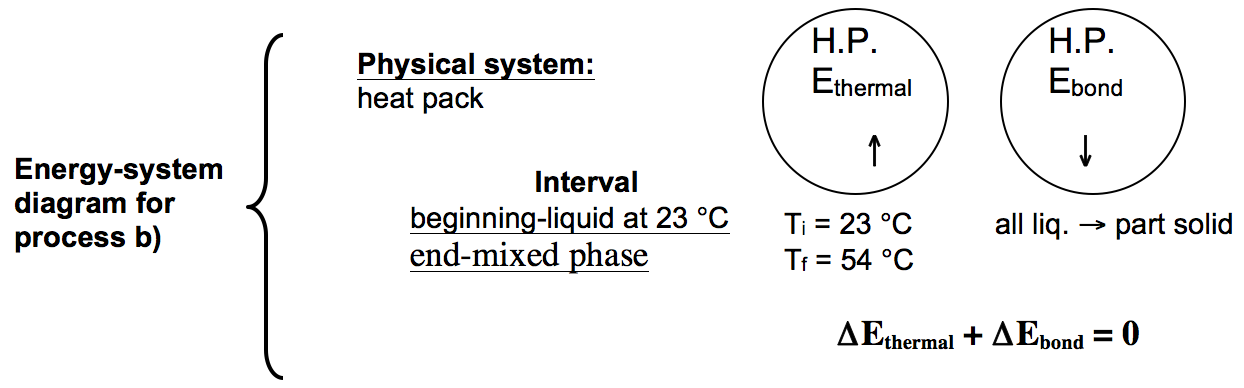
\includegraphics[width=\linewidth]{act115-chi}
	}

\WCD
\note{Pose the Question}{
	So where did the energy come from when the clicker is clicked?
	
	And: How do you know?
	
	Have the class answer this, making sure they can explain and how they know where it came from.
	
	Ans: Observe the partial phase change (bonds getting made) and $T$ going up; clicker adds insignificant energy
}

	\bitem {Getting back to room temperature}
	
	If you now partially remove the bubble wrap so the heat pack can exchange energy with the environment, sketch the rest of the path that gets the heat pack back to a solid at room temperature. Should this path fall ``on top of'' the heating path?
	
	\note{}{
		The \ThreePhaseModel{} assumes that in a mixed state, the two phases are in thermal equilibrium. After the heat pack is triggered it the temperature quickly increases to close to the melting point during initial solidification, but because the complete solidification process doesn't happen quickly (it involves hydration) the heat pack is typically far from being in thermal equilibrium as it cools from the melting temperature to room temperature. But, if we imagine it is still fairly well insulated, then the model prediction that it follows the standard horizontal line at the melting temperature until it is completely solidified would describe how a heat pack behaves. So, to the extent that the model applies to the heat pack phenomena of getting from a mixed state at the melting temp back to room temperature, it does so as the model predicts.  
	}
	
	\bitem {\ThreePhaseModel{} with Super-Cooling}
	
	Discuss in your small group how you can summarize the difference in the \ThreePhaseModel{} as applied to situations when there is and when there isn't significant/noticeable supercooling. Put your summary on your board and be ready to explain to the whole class.
	
	\note{}{
		Without supercooling the heating curve and cooling curve are identical.  When there is supercooling, the cooling curve in the liquid region will extend below the melting/freezing temperature. This means the substance can exist in the liquid state even when the temperature is below the freezing temperature. As the temperature is lowered further in the supercooled state, or when the substance is disturbed, it ``jumps'' vertically to the mixed state without absorbing or giving off heat to the environment.  (Note: supercooling also occurs when vapor cools below the boiling/condensation temperature and superheating occurs when a substance in the liquid phase is heated above the boiling point.
	}

\WCD

\end{benumerate}

\note{}{
	Let one or two groups take a stab at explaining the difference in the models with and without supercooling.  Perhaps the best summary is simply to compare the difference in the cooling curves and explain that the heating curves are the same. 
}
